\lab{Nearest Neighbor Search}{Nearest Neighbor Search}
\label{lab:NNS}

\objective{Nearest neighbor search is an optimization problem that arises in applications such as computer vision, pattern recognition, internet marketing, and data compression. In this lab we implement a K-D tree to solve the problem efficiently, then learn use scipy's K-D tree in sklearn to implement a handwriting recognition algorithm.}

\section*{The Nearest Neighbor Search Problem}

Suppose you move into a new city with several post offices.
Since your time is valuable, you wish to know which post office is closest to your home.
This is called the nearest neighbor search problem, and it has many applications.

In general, suppose that $X$ is a collection of data, called a \emph{training set}.
Let $y$ be any point (often called the \emph{target} point) in the same space as the data in $X$.
The nearest neighbor search problem determines the point in $X$ that is closest to $y$.
For example, in the post office problem the set $X$ could be addresses or latitude and longtitude data for each post office in the city.
Then $y$ would be the data that represents your new home, and the task is to find the closest post office in $X$ to $y$.

% Problem 1: Euclidean Distance
\begin{problem}
In order to solve the nearest neighbor search problem we need a way to measure distance.
A function that measures distance between two points is called a \emph{metric}.
The euclidean metric measures the distance between two points in $\mathbb{R}^n$ by
\[
d(x,y) = \sqrt{\displaystyle\sum_{i=1}^n (x_i - y_i)^2} = \| x - y \|_2
\]

Write a function that accepts two $1 \times k$ numpy arrays and returns the euclidean distance between them.
Raise a \li{ValueError} if the vectors don't have the same dimension.
\end{problem}

Consider again the post office example.
One way to find out which post office is closest is to drive from home to each post office, measure the mileage, and then choose the post office that is the closest.
This is called an exhaustive search.
More precisely, we measure the distance of $y$ to each point in $X$, and choose the point with the smallest distance.
This method is ineffecient however, and only feasible if the training set is very small.

% Problem 2: Exhaustive search method
\begin{problem}
Write a function that solves the nearest neighbor search problem by exhaustively checking all of the distances between a given point and each point in a data set.
The function should take in a set of data points (as an $m \times k$ numpy array) and a single target point (as a $1 \times k$ numpy array).
Return the point in the training set that is closest to the target point and its distance from the target.

The complexity of this algorithm is $O(mk)$, where $k$ is the number of dimensions and $m$ is the number of data points.
\end{problem}

\section*{K-D Trees}

A \href{https://en.wikipedia.org/wiki/K-d_tree}{\emph{$k$-d tree}} is a special kind of binary search tree\footnote{This lab is a sequel to the Data Structures II lab, and should not be attempted until the reader has successfully implemented a binary search tree in Python.} for high dimensional data (i.e., more dimensions than 1).
While a binary search tree excludes regions of the number line from a search until the search point is found, a $k$-d tree works on regions of $\mathbb{R}^k$.
So long as the data in the tree meets certain dimensionality requirements, similar efficiency gains may be made.

Recall that to search for a point in a binary search tree, we start at the root, and if the point we are searching for is less than the root we proceed down the left branch of the tree.
If it is larger we proceed down the right branch.
By doing this, we exclude a region of the number line (and therefore the subtree in the opposite direction) from our search.
By eliminating this region from consideration, we have far fewer points to search and the efficiency of our search is greatly increased.
%See Figure \ref{fig:k-binary-search} for an illustration.

Like a binary search tree, a $k$-d tree starts with a root node with a depth, or level, of 0.
At the $i^{th}$ level, the nodes to the left of a parent have a lower value in the $i^{th}$ dimension.
Nodes to the right have a greater value in the $i^{th}$ dimension.
At the next level, we do the same for the next dimension.
For example, consider data in $\mathbb{R}^3$.
The root node partitions the data according to the first dimension.
The children of the root partition according to the second dimension, and the grandchildren along the third.
See Figure \ref{fig:k-binary-search} for an example in $\mathbb{R}^2$.

As with any other data structure, the first task is to construct a node class to store data.
A \li{KDTNode} is similar to a \li{BSTNode}, except it has another attribute called \li{axis}.
The \li{axis} attribute tells us which dimension of $\mathbb{R}^k$ to split on.

\begin{figure}[H]
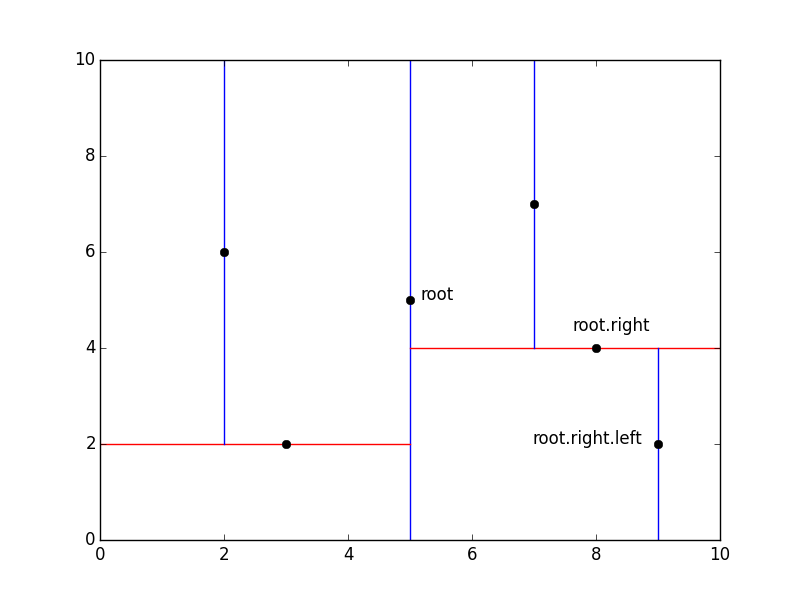
\includegraphics[width=\textwidth]{kdpic1.png}
\caption{A regular binary search tree partitions $\mathbb{R}$, but a $k$-d tree partitions $\mathbb{R}^{k}$. The above graph illustrates the partition for a $k$-d tree loaded with the points (5, 5), (8, 4), (3, 2), (7, 7), (2, 6), and (9, 2), in that order. To find the point (9, 2), we start at the root. Since the $x$-coordinate of (9, 2) is greater than the $x$-coordinate of (5, 5), we move into the region to the right of the middle blue line, thus excluding all points ($x$, $y$) with $x < 5$. Next we compare (9, 2) to the root's right child, (8, 4). Since the $y$-coordinate of (9, 2) is less than the $y$-coordinate of (8, 4), we move below the red line on the right, thus excluding all points ($x$, $y$) with $y > 4$. We have now found (9, 2), since it is the left child of (8, 4).}
\label{fig:k-binary-search}
\end{figure}

% KDT Node class
\begin{lstlisting}
from Trees import BSTNode

class KDTNode(BSTNode):
    """Node class for K-D Trees. Inherits from BSTNode.
    Attributes:
        left (KDTNode): a reference to this node's left child.
        right (KDTNode): a reference to this node's right child.
        parent (KDTNode): a reference to this node's parent node.
        data (ndarray): a coordinate in k-dimensional space.
        axis (int): the dimension to make comparisons on.
    """
    def __init__(self, data):
        """Construct a K-D Tree node containing 'data'. The left, right,
        and prev attributes are set in the constructor of BSTNode.
        """
        BSTNode.__init__(self, data)
        self.axis  = 0
\end{lstlisting}

% Problem 3: KDTNode
\begin{problem}
Import the \li{BSTNode} class from \texttt{Trees.py}%\footnote{The file \texttt{Trees.py} is part of the Data Structures II lab.}
Write a \li{KDTNode} class that inherits from \li{BSTNode}.
\begin{enumerate}
\item Modify the constructor so that a \li{KDTNode} can only hold a numpy array (\li{np.ndarray}).
If any other data type is given, raise a \li{TypeError}.
\item Write the \li{__sub__} magic method so that \li{x} - \li{y} returns the euclidean distance between the data in node \li{x} and the data in node \li{y}.

\item Write the \li{__eq__} magic method so that \li{x == y} is \li{True} if and only if \li{x} and \li{y} have the same data (Hint: \li{np.allclose()})

\item Finally, write the \li{__lt__} and \li{__gt__} magic methods so that the $<$ and $>$ operators compare the $i^{th}$ entry of the data, where $i$ is the \li{axis} attribute of the node on the \emph{right side} of the operator.
For example,

\begin{lstlisting}
>>> x = KDTNode(np.array([1,2]))
>>> y = KDTNode(np.array([3,1]))
>>> y.axis = 0			# Compare the '0th' entry of the data 
>>> x < y				# True, since 1 < 3
True
>>> x > y
False

>>> y.axis = 1			# Compare the '1st' entry of the data
>>> x < y				# False, since 2 > 1
False
>>> x > y
True
\end{lstlisting}
\end{enumerate}
\end{problem}

Now we construct the $k$-d tree class.
%The constructor accepts a set of data as an $m \times k$ numpy array and inserts each $1 \times k$ point into the tree.
For an optimal $k$-d tree, the data needs to be inserted in a very particular order.
However, inserting at random still usually produces a good tree.
Here we simply insert the data in the order that it is given.

The major difference between a $k$-d tree and a binary search tree is how the data is compared at each depth level.
This is simplified by using the magic methods in the \li{KDTnode} class.
Though we don't need to use a \li{find} method in solving the nearest neighbor problem, we provide the $k$-d tree version of \li{find} as an instructive example.

In the \li{find} method, every comparison in the recursive \li{_step} function compares the data of \li{target} and \li{current} based on the \li{axis} attribute of \li{current}, since it is on the right-hand side of the expression.
This way if each existing node in the tree has the correct \li{axis}, the correct comparisons are made as we descend the tree.

\begin{comment}
    def __init__(self, data_set):
        """Set the k attribute and fill the tree with the points in 'data_set'.

        Raises:
            TypeError: 'data_set' is not a numpy array (of type np.ndarray).
        """

        # Validate the input type.
        if not isinstance(data_set, np.ndarray):
            raise TypeError("data_set must be a numpy array.")

        # Set the root and dimension attributes.
        BST.__init__(self)
        self.k = data_set.shape[1]

        # Load the data in one point at a time.
        for point in data_set:
            self.insert(point)
\end{comment}

\begin{lstlisting}
from Trees import BST

class KDT(BST):
    """A k-dimensional binary search tree object.
    Used to solve the nearest neighbor problem efficiently.
    Attributes:
        root (KDTNode): the root node of the tree. Like all other
            nodes in the tree, the root houses data as a numpy array.
        k (int): the dimension of the tree (the 'k' of the k-d tree).
    """

	def find(self, data):
        """Return the node containing 'data'.
        
        Raises:
            ValueError: there is node containing 'data' in the tree,
                or the tree is empty.
        """

        # First check that the tree is not empty.
        if self.root is None:
            raise ValueError(str(data) + " is not in the tree.")
		
        # Define a recursive function to traverse the tree.
        def _step(current, target):
            """Recursively approach the target node."""
            
            if current is None:             # Base case: target not found.
                return current
            if current == other:            # Base case: target found!
                return current
            if target < current:            # Recursively search to the left.
                return _step(current.left, target)
            else:                           # Recursively search to the right.
                return _step(current.right, target)
        
        # Create a new node to use the KDTNode comparison operators.
        n = KDTNode(data)

        # Call the recursive function, starting at the root
        found = _step(self.root, n)
        if found is None:                   # Report the data was not found.
            raise ValueError(str(data) + " is not in the tree.")
        return found                        # Othewise, return the target node.
\end{lstlisting}

% Problem 4: Implement the K-D Tree!
\begin{problem}
Finish implementing the \li{KDT} class.
\begin{enumerate}
\item Override the \li{insert} method.
To insert a new node, find the correct insertion point by recursively descending through the tree as in the \li{find} method (see figure \ref{fig:k-insert} for an example).
%Note that the $k$ attribute will have to be set at some point.

The \li{axis} attribute of the new node will be one more than that axis of the parent node.
If the last dimension of the data has been reached, start over at the first dimension.

\item To solve the nearest neighbor search problem, we need only create the $k$-d tree once.
Then we can use it multiple times with different target points.
To prevent the user from altering the tree, disable the \li{remove} method.
Raise a \li{NotImplementedError} if the method is called, and allow it to receive any number of arguments.
\end{enumerate}
\end{problem}

\begin{figure}[H]
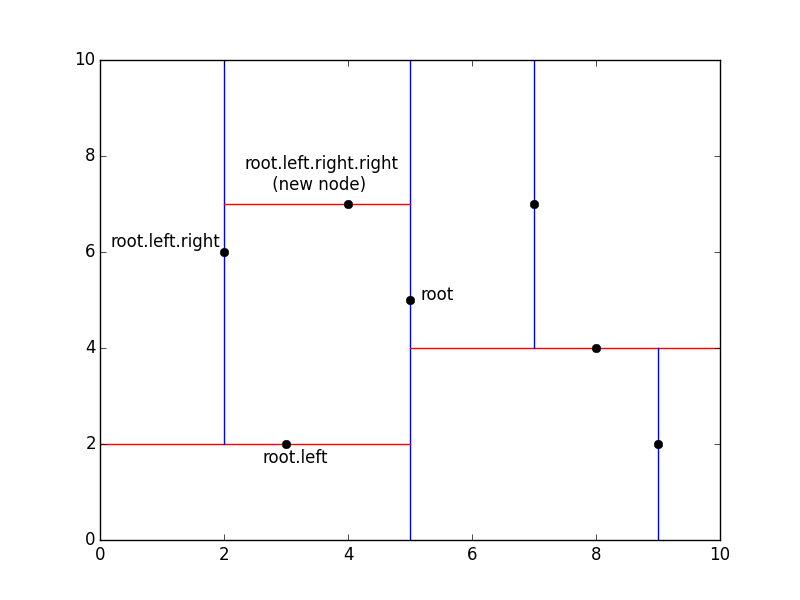
\includegraphics[width=\textwidth]{kdpic2.png}
\caption{To insert the point (4, 7) into the $k$-d tree of figure \ref{fig:k-binary-search}, we find the node that will be the new node's parent. Start at the root, (5, 5). Since the $x$-coordinate of (4, 7) is less than the $x$-coordinate of (5, 5), we move into the region to the left of the middle blue line, to the root's left child, (3, 2). The $y$-coordinate of (4, 7) is greater than the $y$-coordinate of (3, 2), so we move above the red line on the left, to the right child (2, 6). Now we return to comparing the $x$-coordinates, and since $4 > 2$ and (2, 6) has no right child, we install (4, 7) as the right child of (2, 6).}
\label{fig:k-insert}
\end{figure}

Using a $k$-d tree to solve the nearest neighbor search problem requires some care.
At first glance, it appears that a procedure similar to \li{find} or \li{insert} will immediately yield the result.
However, this is not always the case (see Figure \ref{fig:bad-search}).

To correctly find the nearest neighbor we will keep track of the target point, the current search node, current best point, and current minimum distance.
Start at the root node.
Then the current search node and current best point will be root, and the current minimum distance will be the euclidean distance from \li{root} to \li{target}.
We then proceed recursively as in the \li{search} method.
As we find better current best points, we update the appropriate variables accordingly.

Once we have reached the bottom of the tree, we will have a good guess for the nearest neighbor.
However, we are not guaranteed to have arrived at the correct point.
One way to ensure that we have arrived at the correct point is to draw a hypersphere with a radius of the current minimum distance around the candidate nearest neighbor.
If this hypersphere does not intersect any of the hyperplanes that split the $k$-d tree, then we know that have found a best point.

\begin{figure}[H]
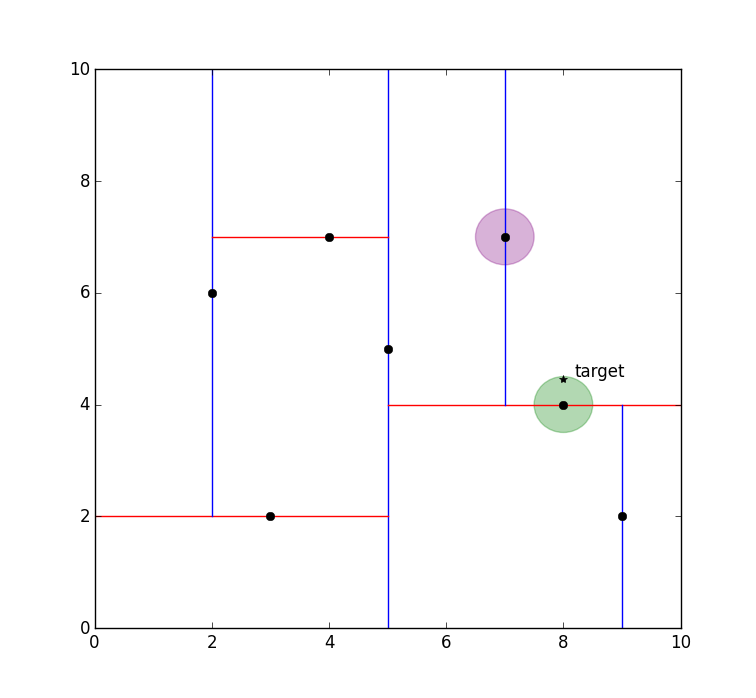
\includegraphics[width=\textwidth]{kdpic3.png}
\caption{Suppose we want to find the point in the $k$-d tree of figure \ref{fig:k-insert} that is closest to (8, 4.5). First we record the distance from the root to the target as the current minimum distance (about 3.04), then travel down the tree to the right. The right child, (8, 4), is only .5 units away from the target (the green circle), so we update the minimum distance. Since (8, 4) is not a leaf in the tree, we could continue down to the left child, (7, 7). However, this leaf node is much further from the target (the purple circle). To ensure that we terminate the algorithm correctly we check to see if the hypersphere of radius .5 around the current node (the green circle) intersects with any other hyperplanes. Since it does not, we stop descending down the tree and conclude (correctly) that (8, 4) is the nearest neighbor.}
\label{fig:bad-search}
\end{figure}

\begin{comment}
\begin{figure}
\caption{We need a figure here.  Something similar to what is found at http://web.stanford.edu/class/cs106l/handouts/assignment-3-kdtree.pdf, page 8.  This needs a great caption.  I can write it when the figure is done. Of course we will need to have a reference to this document.}
\label{fig:hyperplanes}
\end{figure}
\end{comment}

While we can not easily draw the correct hypersphere, there is an equivalent procedure that has a straightforward implementation in python.
Before we finally decide to descend in one direction, we add the minimum distance to the $i^{th}$ entry of the target point's data, where $i$ is the \li{axis} of the candidate nearest neighbor.
If this sum is greater that the $i^{th}$ entry of the current search node, then the hypersphere would necessarily intersect one of the hyperplanes drawn by the tree (why?).

We summarize the algorithm below.

\begin{algorithm}
\begin{algorithmic}[1]
\Procedure{KDTSearch}{current, target, neighbor, distance}
\If {current is None}
    \State return neighbor, distance (Base Case)
\EndIf
\State index = current.axis
\State d = euclidean\_distance
	\If {d(current,target) $<$ distance}
		\State neighbor = current
		\State distance = d(current,target)
	\EndIf
	\If {target.data[index] $<$ current.data[index]}
		\State neighbor, distance = KDTSearch(current.left, target,
			\State									neighbor, distance)
		\If {target.data[index] + distance $>=$ current.data[index]}
			\State neighbor, distance = KDTSearch(current.right, target,
				\State									neighbor, distance)
		\EndIf
	\Else
		\State neighbor, distance = KDTSearch(current.right, target,
			\State									neighbor, distance)
		\If {target.data[index] - distance $<=$ current.data[index]}
			\State neighbor, distance = KDTSearch(current.left, target,
				\State									neighbor, distance)
		\EndIf
	\EndIf
\State return neighbor, distance
\EndProcedure
\end{algorithmic}
\caption{$k$-d tree nearest neighbor search}
\label{alg:kdneighborz}
\end{algorithm}


\begin{problem}
Use Algorithm \ref{alg:kdneighborz} to write a function that solves the nearest neighbor search problem by searching through a $k$-d tree (your \li{KDT} object).
The function should take in a data set and a single target point.
Return the nearest neighbor in the data set and the distance from the nearest neighbor to the target point, as in Problem 2.

To test your function, use Scipy's built-in \li{KDTree} object.
This structure behaves like the \li{KDT} class, but its operations are heavily optimized.
To solve the nearest neighbor problem, initialize the tree with data, then `query' the tree with the target point.
The \li{query} method returns a tuple of the minimun distance and the index of the nearest neighbor in the data.

\begin{lstlisting}
>>> from scipy.spatial import KDTree

# Initialize the tree with data (in this example we use random data).
>>> data = np.random.random((100,5))
>>> target = np.random.random(5)
>>> tree = KDTree(data)

# Query the tree and print the minimum distance.
>>> min_distance, index = tree.query(target)
>>> print(min_distance)
0.309671532426

# Print the nearest neighbor by indexing into the tree's data.
>>> print(tree.data[index])
[ 0.68001084  0.02021068  0.70421171  0.57488834  0.50492779]
\end{lstlisting}
\end{problem}

\section*{Application: Handwriting Recognition}

\subsection*{Classification}

Suppose that we are given a training set of data as well as a set of \emph{labels} that describe each datum in the training set.
For example, suppose that we had a training set containing the incomes and debt levels of $N$ individuals.
Along with this data, we have a set $N$ labels that state whether the individual has filed for bankruptcy.
The classification problem is to try and assign the correct label to an unlabelled data point.

\subsection*{$k$-Nearest Neighbors}

In our previous work, we used a $k$-d tree to find the nearest neighbor of a target point.
A more general problem is to find the \emph{k} nearest neighbors to a point (using some metric to measure ``distance'' between data points).
In classification, we find the $k$ nearest neighbors, we let each neighbor ``vote'' to decide what label to give the new point.
For example, consider the bankrupty case in the previous section.
If we find the 10 nearest neighbors to a new individual, and 8 of them went bankrupt, then we would predict that the individual will also go bankrupt.
On the other hand, if 7 of the nearest neighbors had not filed for bankruptcy, we would predict that the individual was at low risk for bankruptcy.

\subsection*{The Handwriting Recognition Problem}

The problem of recognizing handwritten letters and numbers with a computer has many applications.
A computer image may be thought of a vector in $\mathbb{R}^n$, where $n$ is the number of pixels in the image and the entries represent how bright each pixel is.
If two people write the same number, we would expect the vectors representing a scanned image of those number to be close in the euclidean metric.
This insight means that given a training set of scanned images along with correct labels, we may confidently infer the label of a new scanned image.

\subsection*{scipy.sklearn}

%More information about this package can be found at http://scikit-learn.org/stable/modules/neighbors.html.
The \li{sklearn} module in \li{scipy} contains powerful tools for solving the nearest neighbor problem.
To start nearest neighbors classification, we import the neighbors module from sklearn.
This module has a class for setting up a k-nearest neighbors classifier.
\begin{lstlisting}
# Import the neighbors module
>>> from sklearn import neighbors

# Create an instance of a k-nearest neighbors classifier.
# 'n_neighbors' determines how many neighbors to give votes to.
# 'weights' may be 'uniform' or 'distance.'  The 'distance' option
#     gives nearer neighbors more weight.
# 'p=2' instructs the class to use the euclidean metric.
>>> nbrs = neighbors.KNeighborsClassifier(n_neighbors=8, weights='distance', p=2)
\end{lstlisting}

The \li{nbrs} object has two useful methods for classification.
The first, \li{fit}, will take arrays of data (the training set) and labels and put them into a $k$-d tree.
This can then be used to find k-nearest neighbors, much like the \li{KDT} class that we implemented previously.

\begin{lstlisting}
# 'points' is some numpy array of data
# 'labels' is a numpy array of labels describing the data in points.
>>> nbrs.fit(points, labels)
\end{lstlisting}

The second method, \li{predict}, will do a k-nearest neighbor search on the $k$-d tree and use the result to attach a label to unlabelled points.

\begin{lstlisting}
# 'testpoints' is an array of unlabeled points.
# Perform the search and calculate the accuracy of the classification.
>>> prediction = nbrs.predict(testpoints)
>>> np.average(prediction/testlabels)
\end{lstlisting}

\begin{problem}
The United States Postal Service has made a collection of labelled hand written digits available to the public, provided in \li{PostalData.npz}.
We will use this data for k-nearest neighbor classification.
This data set may be loaded by using the following command:
\begin{lstlisting}
labels, points, testlabels, testpoints = np.load('PostalData.npz').items()
\end{lstlisting}
This contains a training set and a test set.
The first entry of each array is a name, so \li{points[1]} and \li{labels[1]} are the actual points and labels to use.
Each point is an image that is represented by a flattened $28 \times 28$ matrix of pixels. 
The corresponding label indicates which number was written.

Classify the testpoints with \li{n_neighbors} as 1, 4 or 10, and with \li{weights} as \li{'uniform'} or \li{'distance'}.
For each trial print a report indicating how your classifier performs in terms of percentage of correct classifications.
Which combination gives the most correct classifications?
(Hint: define an inner function that takes in \li{n_neighbors} and \li{weights} as arguments calls the neighbors functions appropriately)

A similar classification process is used by the United States Postal Service to automatically determine the zip code to send a letter to.

\begin{figure}[H]
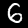
\includegraphics[width=.25\textwidth]{Example.png}
\caption{An example of the number 6 taken from the data set}
\end{figure}
\end{problem}
